% !TEX program = xelatex
\documentclass[UTF8,a4paper,11pt]{ctexart}

\usepackage[a4paper,margin=2.45cm,headheight=15pt]{geometry}
\usepackage{amsmath,amssymb,bm}
\usepackage{booktabs,longtable,tabularx,array}
\usepackage{graphicx}
\usepackage{tikz}
\usetikzlibrary{arrows.meta,positioning,calc}
\usepackage{caption}
\usepackage{enumitem}
\usepackage{fancyhdr}
\usepackage{microtype}
\usepackage{xurl}
\usepackage[hidelinks]{hyperref}

\captionsetup{font=small,labelfont=bf,skip=6pt}
\setlist[itemize]{topsep=3pt,itemsep=2pt,parsep=0pt}
\setlist[enumerate]{topsep=3pt,itemsep=2pt,parsep=0pt}
\setlength{\parindent}{2em}
\setlength{\parskip}{0.3em}
\setlength{\emergencystretch}{3em}
\allowdisplaybreaks

\newcolumntype{L}[1]{>{\raggedright\arraybackslash}p{#1}}
\newcolumntype{Y}{>{\raggedright\arraybackslash}X}
\newcommand{\code}[1]{\texttt{\detokenize{#1}}}
\newcommand{\pathref}[1]{\path{#1}}
\newcommand{\PyQCU}{\mbox{PyQCU}}
\newcommand{\QUDA}{\mbox{QUDA}}

\pagestyle{fancy}
\fancyhf{}
\fancyhead[L]{\small High-Performance Multigrid for Lattice QCD}
\fancyhead[R]{\small Zhang Xin}
\fancyfoot[C]{\thepage}
\renewcommand{\headrulewidth}{0.4pt}

\title{\bfseries High-Performance Implementation of Multigrid Solver\\[0.35em]
for Lattice QCD}
\author{张鑫\\中国科学院近代物理研究所}
\date{2026 年 9 月 28 日}

\begin{document}

\maketitle
\thispagestyle{empty}

\begin{abstract}
传播子求解是格点量子色动力学（Lattice QCD）数值计算的核心瓶颈之一。
本文介绍 PyQCU 中面向 Wilson--Clover 费米子的 CUDA--C++ 多重网格
（MultiGrid, MG）实现。方法以奇偶预处理后的 Dirac 算子为细层问题，
通过低模探测、局部正交聚集、转移算子构造和 Galerkin 投射生成递归粗层；
Strict 路径采用
\[
D_l=X_l+H_l,\qquad
\widehat D_l=X_l^{-1}D_l,\qquad
D_{l+1}=R_l\widehat D_lP_l,
\]
并保留粗层 full geometry 与 \(X/Y/\widehat Y\) 资产。CUDA--C++ 后端
结合五流执行、设备端标量、内核融合、CUDA Graph、分块/着色 Galerkin
构造、持久工作区、校验缓存和非阻塞向量 halo，以降低细层带宽、粗层延迟
和分布式通信成本。性能评价严格采用 \code{git tag test27} 的最终
capacity-aware 数据：请求矩阵包含 72 个 combined 单元，实际完成 66 个
精确单元和 132 条 side record；其余 6 个双 P100 \code{c64}
\(16\times32\times32\times48\) 请求项因显存或 570 s 时限被显式替代。
66 个精确单元的整体中位时间比
\(R=t_{\QUDA}/t_{\PyQCU}=1.025\)，MG-2/3 在 35/44 个单元中更快；
若只采用正式 trace-off 口径，MG 为 21/22 个单元有利。全部精确单元
均通过独立 full-operator 真残差门，PyQCU 与 QUDA 的最大真残差分别为
\(7.40\times10^{-7}\) 和 \(7.97\times10^{-7}\)。结果支持
“MG 专项性能已达到国际先进实现同量级并具有明显场景优势”，但不支持
将结论外推为全部求解器、全部格点或全部并行拓扑上的普遍领先。
\end{abstract}

\noindent\textbf{关键词：}格点量子色动力学；Wilson--Clover 费米子；
多重网格；Galerkin 投影；CUDA；MPI；高性能计算

\section{引言}

\subsection{研究背景}

格点 QCD 通过离散化欧几里得时空上的夸克和胶子场，为非微扰强相互作用
计算提供第一性原理框架。在传播子、关联函数和部分子分布函数等计算中，
最耗时的步骤通常是求解具有特殊结构的稀疏复线性系统
\begin{equation}
 D(U,m_0)\psi=\eta,
\label{eq:propagator}
\end{equation}
其中 \(D\) 为 Wilson 或 Clover 改进的 Wilson--Dirac 算子，\(U\) 为
\(SU(3)\) 规范链接，\(m_0\) 为格点裸质量，\(\eta\) 为源场。
轻夸克质量使 \(D\) 接近奇异，Krylov 方法在低频模态上的收敛随格点体积
恶化，即所谓 critical slowing down。多重网格通过显式构造低模粗空间，
将低频误差转移到粗层处理，从而降低迭代次数对体积的依赖。

\subsection{本文范围}

本文关注 PyQCU 的 MultiGrid 求解器及其 CUDA--C++ 实现，内容分为四条
主线：
\begin{enumerate}
  \item 给出 Wilson/Clover 算子、原始 Dslash 和奇偶 Schur 消元的统一
        数学约定；
  \item 说明自适应聚集多重网格的构造，以及其在 Clover--Wilson
        非正规算子上的特化；
  \item 分析 CUDA--C++ 后端的并行与内存优化；
  \item 基于 \code{test27} 最终数据，对 PyQCU Strict MG 与 QUDA 1.1.0
        MultiGrid 进行严格对照，并明确适用边界。
\end{enumerate}

\subsection{证据与口径}

本文的性能结论只使用 \code{git tag test27} 及其
\pathref{data/report_multigrid_comprehensive_20260928/final_protocol}
中的原始记录。实现分析同时参考当前 CUDA--C++ 源码和
\pathref{docs/report_*.tex} 中的最新技术报告。历史报告中的旧分母或
实验性加速比不再作为最终性能结论；若引用历史版本，只用于说明实现演进
或失败边界。

\section{格点 QCD 传播子与 Dirac 算子}

\subsection{Wilson 作用量和 Dslash}

规范链接 \(U_{x,\mu}\in SU(3)\) 连接格点 \(x\) 与 \(x+\hat\mu\)。
正向和反向协变平移分别为
\begin{equation}
 T_{+\mu}\psi_x=U_{x,\mu}\psi_{x+\hat\mu},\qquad
 T_{-\mu}\psi_x=U^\dagger_{x-\hat\mu,\mu}\psi_{x-\hat\mu}.
\label{eq:covariant-shift}
\end{equation}
取 Wilson 参数 \(r=1\)，定义无质量尺度因子的跃迁核 \(H\)：
\begin{equation}
 (H\psi)_x=
 \sum_{\mu=0}^{3}\left[
 (1-\gamma_\mu)U_{x,\mu}\psi_{x+\hat\mu}
 +(1+\gamma_\mu)U^\dagger_{x-\hat\mu,\mu}\psi_{x-\hat\mu}
 \right].
\label{eq:hopping-kernel}
\end{equation}
相应的 Wilson 费米子部分和作用量为
\begin{align}
 D_W&=(m_0+4)I-\frac{1}{2}H
 =(m_0+4)\left(I-\kappa H\right),
\label{eq:wilson-operator}\\
 S_W&=\sum_x\bar\psi_xD_W\psi_x,
\qquad
 \kappa=\frac{1}{2m_0+8}.
\label{eq:wilson-action}
\end{align}
因此
\begin{equation}
 m_0+4=\frac{1}{2\kappa}.
\label{eq:kappa-identity}
\end{equation}
PyQCU 求解器中常用的预条件归一化形式为
\begin{equation}
 D_{\mathrm{pc}}=I-\frac{\kappa}{u_0}H,
\qquad
 D_W=(m_0+4)D_{\mathrm{pc}},
\label{eq:wilson-pc}
\end{equation}
其中 \(u_0\) 为 tadpole 因子。当前 C++ 生产路径等价于 \(u_0=1\)。
需要强调的是，C++ 原始 Wilson-Dslash 入口返回的是裸核 \(H\)，不含
单位项和 \(-\kappa\) 因子；带单位项的 Python 入口则返回
\(I-(\kappa/u_0)H\)。在跨实现比较时，必须显式保持该归一化差异。

\subsection{Clover 改进}

Clover 项通过局域四点规范环改进 Wilson 算子的 \(O(a)\) 误差。
定义有向 plaquette
\begin{equation}
 P_{\mu\nu}(x)=
 U_\mu(x)U_\nu(x+\hat\mu)
 U^\dagger_\mu(x+\hat\nu)U^\dagger_\nu(x),
\label{eq:plaquette}
\end{equation}
以及四叶 Clover 和
\begin{equation}
 Q_{\mu\nu}=P_{\mu\nu}+P_{\nu,-\mu}
 +P_{-\mu,-\nu}+P_{-\nu,\mu},\qquad
 C_{\mu\nu}=Q_{\mu\nu}-Q^\dagger_{\mu\nu}.
\label{eq:clover-loop}
\end{equation}
当前代码级 onsite 修正块为
\begin{equation}
 T_p=-\frac{\kappa c_{\mathrm{sw}}}{8u_0}
 \sum_{\mu<\nu}\gamma_\mu\gamma_\nu C_{\mu\nu},
 \qquad
 A_p=I_p+T_p,
\label{eq:clover-block}
\end{equation}
其中有效 \(c_{\mathrm{sw}}=1\)。预条件归一化和物理归一化算子分别为
\begin{align}
 D^C_{\mathrm{pc}}&=I-\frac{\kappa}{u_0}H+T,
\label{eq:clover-pc}\\
 D^C_{\mathrm{phys}}&=(m_0+4)I-\frac{1}{2}H
 -\frac{c_{\mathrm{sw}}}{16u_0}
 \sum_{\mu<\nu}\gamma_\mu\gamma_\nu C_{\mu\nu}.
\label{eq:clover-phys}
\end{align}
Clover 项不扩大最近邻 stencil，但把每个格点的局域自由度由纯颜色空间
提升为 \(4\times3=12\) 维 spin--color 空间。其逆或分解必须在细层和
粗层算子构造中批量执行。

\subsection{奇偶分块与 Schur 消元}

将场按格点奇偶性划分为 even 和 odd 两个子空间。归一化 Clover 算子
可以写成
\begin{equation}
 D_{\mathrm{pc}}=
 \begin{pmatrix}
 A_e & -\kappa H_{eo}\\
 -\kappa H_{oe} & A_o
 \end{pmatrix},
\qquad
 A_p=
 \begin{cases}
 I_p, & \text{Wilson},\\
 I_p+T_p, & \text{Clover}.
 \end{cases}
\label{eq:even-odd-block}
\end{equation}
以奇数子格 Schur 补为例，消去 even 分量后得到
\begin{align}
 S_o&=A_o-\kappa^2H_{oe}A_e^{-1}H_{eo},
\label{eq:schur}\\
 b_o^{\mathrm{pc}}&=b_o+\kappa H_{oe}A_e^{-1}b_e,
\label{eq:schur-rhs}\\
 x_e&=A_e^{-1}\left(b_e+\kappa H_{eo}x_o\right).
\label{eq:schur-reconstruct}
\end{align}
对于 Wilson 算子，\(A_e=A_o=I\)，因此
\begin{equation}
 S_o=I-\kappa^2H_{oe}H_{eo}.
\label{eq:wilson-schur}
\end{equation}
该变换是精确消元：外层 Krylov 求解只作用于半体积未知量，收敛后再重建
另一半。最终正确性仍由完整 Wilson/Clover 算子的真残差判定，而不是由
Schur 子系统的递推残差代替。

\section{多重网格算法与 QCD 特化}

\subsection{低模粗空间与 Galerkin 投影}

多重网格的目标是将误差分解为高频与低频两部分：
\begin{equation}
 e=e_{\mathrm{high}}+e_{\mathrm{low}}.
\label{eq:error-split}
\end{equation}
平滑器负责压低高频误差，粗空间负责表示低频误差。设第 \(l\) 层算子为
\(A_l\)，近零模集合满足
\begin{equation}
 A_lB_l\approx 0.
\label{eq:near-null}
\end{equation}
\(B_l\) 不是精确核，而是低模空间的数值近似。将 \(B_l\) 按 aggregate
重排并在每个 aggregate 内做正交化，得到延拓算子 \(P_l\)，并定义限制
算子
\begin{equation}
 R_l=P_l^\dagger.
\label{eq:restriction}
\end{equation}
局部正交化满足
\begin{equation}
 P_l^\dagger P_l=I.
\label{eq:local-orthogonality}
\end{equation}
粗层算子则由 Galerkin 投影给出：
\begin{equation}
 A_{l+1}=R_lA_lP_l.
\label{eq:galerkin}
\end{equation}
对于非 Hermitian 或非正规算子，\(P_lP_l^\dagger\neq I\)，因此粗空间
不能替代细层单位算子。粗层的正确作用是消除 \(P_l\) 可表示的低模误差，
而不是重新定义一个等价的细层问题。

\subsection{格点 QCD 中多重网格为何困难}

格点 QCD MG 面临三类相互耦合的约束。

\paragraph{隐式稀疏矩阵不可显式存储。}
在代表性较粗层中，若粗自由度为 \(E\)，粗格点数记为 \(N_c\)，则完整
矩阵维度为 \(EN_c\)，显式存储需要
\begin{equation}
 O\left((EN_c)^2\right)
\label{eq:dense-scaling}
\end{equation}
个复数。对于一个 \(N_c\approx49152\)、\(E=24\) 的层级，
\(EN_c\approx1{,}179{,}648\)；complex64 稠密矩阵约为 11.1 TB，
complex128 约为 22.3 TB。实际实现只能保存有限支撑的 block/stencil，
并通过 matrix-free 或打包资产应用算子。

\paragraph{Setup 是高强度数值构造。}
粗层资产不仅包含一次矩阵乘法，还包括近零模生成、局部正交化、
\(P/R\) 构造、Galerkin probing、onsite 逆和 \(\widehat Y\) 生成。
这些步骤涉及多次 full-field matvec、投影、缓存读写和显存峰值控制。
若 setup 无法摊销到足够的求解次数，MG 即使减少外层迭代也可能没有
端到端收益。

\paragraph{粗层是延迟问题，而非算术问题。}
粗层自由度数较小，但每次 V-cycle 都包含多次点积、向量更新、
halo 交换和同步。小内核启动、D2H/H2D 标量传输、MPI 延迟和
host/device 同步会主导 wall time。因此，通用 MG 框架即使算法正确，
直接移植到 GPU 后也可能无法获得实用加速。

\subsection{PyQCU Strict 的 QCD 特化}

PyQCU 当前正式主线为 Strict full-coarse MG。其粗层保留完整几何，
只在细层使用目标 parity 的 compact 表示。令
\begin{equation}
 D_l=X_l+H_l,
\label{eq:strict-split}
\end{equation}
其中 \(X_l\) 收集零位移 onsite block，\(H_l\) 收集轴邻近 block。
左预条件后的算子为
\begin{equation}
 \widehat D_l=X_l^{-1}D_l=I+\widehat H_l,
\qquad
 \widehat H_l=X_l^{-1}H_l.
\label{eq:strict-preconditioned}
\end{equation}
粗层转移满足
\begin{equation}
 D_{l+1}=R_l\widehat D_lP_l
 =R_l\left(X_l^{-1}D_l\right)P_l.
\label{eq:strict-galerkin}
\end{equation}
运行期保存的轴链接资产为
\begin{equation}
 Y^{f}_{l,\mu},\quad Y^{b}_{l,\mu},
\qquad
 \widehat Y^{f}_{l,\mu}=X_l^{-1}Y^{f}_{l,\mu},
\qquad
 \widehat Y^{b}_{l,\mu}=Y^{b}_{l,\mu}X_l^{-\dagger}.
\label{eq:yhat}
\end{equation}
其中 forward 与 backward 的预条件顺序不同。raw \(Y\) 主要作为 setup
和诊断数据，常规求解驻留 \(\widehat Y\)、\(X\) 与 \(X^{-1}\)。

对于细层目标 parity \(p\)，\(R_l\) 将 compact target-parity 残差
映射为 full coarse 向量，\(P_l\) 将 full coarse 修正映射回 compact
目标 parity。粗层资产始终保留 full geometry。该约定避免了用
hopping-only 粗算子替代完整算子的错误，也使 MATPC 与递归粗层求解
使用一致的物理语义。

\begin{figure}[htbp]
\centering
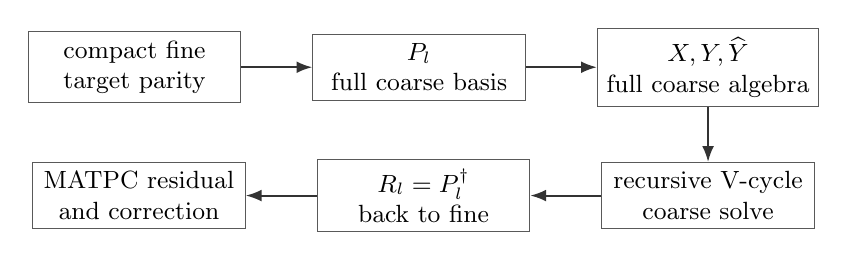
\begin{tikzpicture}[
  node distance=7mm and 9mm,
  box/.style={draw=black!65,fill=white,rectangle,align=center,
    minimum width=2.7cm,minimum height=0.8cm,font=\small},
  arrow/.style={-{Latex[length=2mm]},draw=black!80,line width=0.7pt}
]
  \node[box] (fine) {compact fine\\target parity};
  \node[box,right=of fine] (p) {\(P_l\)\\full coarse basis};
  \node[box,right=of p] (asset) {\(X,Y,\widehat Y\)\\full coarse algebra};
  \node[box,below=of asset] (cycle) {recursive V-cycle\\coarse solve};
  \node[box,left=of cycle] (r) {\(R_l=P_l^\dagger\)\\back to fine};
  \node[box,left=of r] (res) {MATPC residual\\and correction};
  \draw[arrow] (fine) -- (p);
  \draw[arrow] (p) -- (asset);
  \draw[arrow] (asset) -- (cycle);
  \draw[arrow] (cycle) -- (r);
  \draw[arrow] (r) -- (res);
\end{tikzpicture}
\caption{Strict MG 的细层 compact 表示、粗层 full 几何与 \(X/Y/\widehat Y\)
资产之间的数据流。}
\label{fig:strict-flow}
\end{figure}

\subsection{V-cycle、平滑器和外层 FGMRES}

一次 MG 预条件由细层 MR 平滑、restriction、递归粗层求解、prolongation
和 post-smoothing 组成。固定步 MR 更新为
\begin{equation}
 \alpha=\frac{\langle v,r\rangle}{\langle v,v\rangle},
\qquad
 x\leftarrow x+\alpha r,
\qquad
 r\leftarrow r-\alpha v.
\label{eq:mr}
\end{equation}
外层使用右预条件 flexible GMRES。第 \(j\) 个 Arnoldi 列满足
\begin{align}
 z_j&=M_j^{-1}v_j,\qquad w_j=M_pz_j,
\label{eq:fgmres-preconditioner}\\
 x&\leftarrow x+\sum_jz_jy_j,
\label{eq:fgmres-update}
\end{align}
其中每个 \(M_j\) 可以不同，因此可以使用非固定线性的递归 MG 预条件器。
PyQCU 在 restart 边界执行 full-operator 真残差刷新，避免仅依赖递推
标量判定收敛。若 Arnoldi 历史长度为 \(m\)，令 \(B_f\) 表示一个
compact fine 向量、\(B_c\) 表示一个 full first-coarse 向量，则融合
FGMRES 工作区为
\begin{equation}
 B_{\mathrm{work}}=(2m+5)B_f+2B_c.
\label{eq:fgmres-workspace}
\end{equation}
该工作区在同一几何和 restart 配置下复用于后续求解。

\begin{figure}[htbp]
\centering
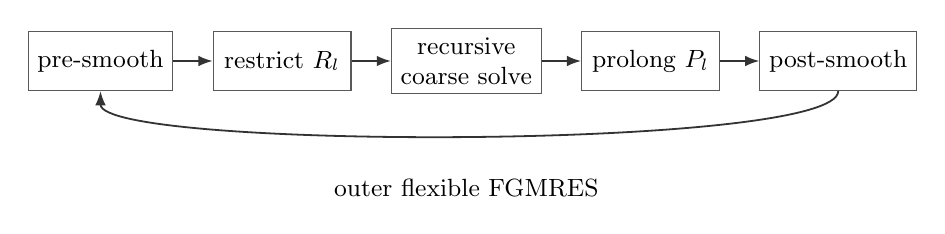
\begin{tikzpicture}[
  node distance=5mm,
  stage/.style={draw=black!65,fill=white,rectangle,align=center,
    minimum width=1.75cm,minimum height=0.75cm,font=\small},
  arrow/.style={-{Latex[length=1.8mm]},draw=black!80,line width=0.65pt}
]
  \node[stage] (pre) {pre-smooth};
  \node[stage,right=of pre] (r) {restrict \(R_l\)};
  \node[stage,right=of r] (coarse) {recursive\\coarse solve};
  \node[stage,right=of coarse] (p) {prolong \(P_l\)};
  \node[stage,right=of p] (post) {post-smooth};
  \draw[arrow] (pre) -- (r);
  \draw[arrow] (r) -- (coarse);
  \draw[arrow] (coarse) -- (p);
  \draw[arrow] (p) -- (post);
  \draw[arrow] (post.south) .. controls +(0,-0.75) and +(0,-0.75) .. (pre.south);
  \node[below=0.95cm of coarse,font=\small] {outer flexible FGMRES};
\end{tikzpicture}
\caption{外层 FGMRES 与内层递归 V-cycle 的嵌套关系。}
\label{fig:vcycle}
\end{figure}

\section{CUDA--C++ 实现与并行优化}

\subsection{分层软件结构}

PyQCU 的 MG 计算路径由四层组成：
\begin{enumerate}
  \item Python 层负责几何、场、缓存身份和求解器编排；
  \item Cython 桥在调用 C++ 前释放 GIL，并使用
        \code{params}/\code{argv}/\code{set_ptrs} 三个扁平数组传递状态；
  \item C++ 层解析层级几何、创建持久 hierarchy、工作区和通信缓冲；
  \item CUDA/MPI 层执行 Dslash、粗层算子、V-cycle、归约和 halo。
\end{enumerate}
Strict 求解的典型生命周期为
\begin{equation}
 \text{setup}\rightarrow
 \text{Strict init}\rightarrow
 \text{repeated V-cycle/FGMRES}\rightarrow
 \text{Strict end}\rightarrow
 \text{release}.
\label{eq:lifecycle}
\end{equation}
相较于 legacy 路径，Strict 路径在全部调用间保持 per-instance
\code{_SET_INDEX_} 不变，并复用同一 hierarchy。

\subsection{细层内核与访存}

Wilson Dslash 单次应用读取四个正向和四个反向邻居。对于每个方向，
\(1\pm\gamma_\mu\) 将四分量旋量投影至两个独立分量，因此 CUDA 内核
可以先做 spin projection，再执行 \(SU(3)\) 矩阵乘法，降低寄存器和
内存压力。时空维置于张量最后四个轴，使相邻格点在线程块内连续，
有利于合并访存。

Clover 项不改变最近邻支持，但要求每个格点读取和应用 \(12\times12\)
onsite 块。细层实现批量构造 Clover、批量求逆并将 \(D_{ee}^{-1}\) 或
其他 onsite 因子复用于算子应用和 Schur 消元。该设计避免逐点调用通用
矩阵逆，并使 Dslash 的主体保持带宽受限而不是控制流受限。

\subsection{粗层求解与主机同步}

粗层向量较小，逐迭代 cublas 调用、D2H/H2D 标量传输和
\code{cudaStreamSynchronize} 往往比算术本身更昂贵。PyQCU 采用以下
措施：
\begin{itemize}
  \item 将 \(\alpha,\beta,\omega,\rho\) 等标量保留在设备端
        \code{device_vals}，减少逐步骤主机往返；
  \item 将 \(\beta\)-更新与 \(\rho\) 保存、\(r/x\) 更新等元素操作融合；
  \item 对固定粗层迭代段使用 CUDA Graph，减少内核启动开销；
  \item 对小最粗层尝试 cooperative fused solve，当向量过大或
        多 rank 条件不满足时回退到逐迭代路径；
  \item 在单 rank 快速路径中增大残差检查间隔，只在稳定检查点读取
        主机标量。
\end{itemize}
这些优化的共同目标是把粗层从 “tiny-kernel latency dominated” 转变为
可摊销、可预算的执行阶段。

\subsection{Setup、显存与缓存}

Galerkin 构造按粗基向量探测 \(P_l^\dagger A_lP_l\) 的列。直接逐列
构造会产生大量 full-field 调用。当前实现采用着色和 site/column
批处理：互不冲突的 source 在同一个 batch 中执行，并根据 workspace
上限自动选择批大小；当显存不足时回退到更保守的 batch。

Strict runtime cache 使用 HDF5 保存 blocked basis、onsite inverse、
\(\widehat Y\) 和必要元数据。缓存 identity 包含格点几何、精度、
层级、blocking 和算子参数；每个 tensor 记录 shape、dtype 和 SHA256。
读取前逐 tensor 校验，写入使用临时文件与原子发布。该机制避免重复
执行小时级 setup，同时防止身份不匹配或内容损坏被静默复用。

\subsection{分布式粗层通信}

在多 rank 模式下，每个 rank 只持有本地粗块。粗层 halo 只需交换
活跃 face，而不是执行完整全量 gather。c64 分布式 vector halo 使用
以下流水线：
\begin{equation}
 \text{active-face pack}
 \parallel \text{local base kernel}
 \rightarrow
 \text{nonblocking MPI}
 \parallel \text{local tail}
 \rightarrow
 \text{remote correction}.
\label{eq:overlap}
\end{equation}
输入就绪 event 由 main stream 记录，交换流完成 pack、pinned-host
staging 和非阻塞 MPI 收发。main stream 先计算不含远端项的局部核，
随后由合并的 correction kernel 加入 remote forward 与 backward
贡献。

该路径改变浮点加法顺序。complex64 分布式路径默认启用 overlap；
complex128 默认关闭，只有显式设置
\code{PYQCU_STRICT_OVERLAP_C128=1} 并重新通过大格真残差和迭代
回归后才允许启用。当前 link halo 仍使用阻塞式 \code{Sendrecv}，
但通过 pointer identity 缓存；device-aware MPI 与 NVSHMEM 路径属于
后续优化范围。

\section{性能评价}

本章的矩阵口径、覆盖统计、时间比、阶段记录、残差、显存和容量替代
结论，均以 \pathref{docs/report_multigrid_quda_pyqcu_20260928.tex}
及其对应的 \code{test27} 原始数据为主要依据；算子构造和实现机制部分
再结合当前 CUDA--C++ 源码与其他技术报告。

\subsection{实验协议}

性能评价采用 QUDA 1.1.0 MultiGrid 作为对照。设备包括单卡
Tesla V100-SXM2-32GB（\code{sm_70}）和双
Tesla P100-PCIE-16GB（\code{sm_60}，process grid
\code{2x1x1x1}）。矩阵覆盖：
\begin{itemize}
  \item 精度：complex64 与 complex128；
  \item 求解：BiCGStab reference、MG-2、MG-3；
  \item trace：on 与 off；
  \item c64 格点：\(8^3\times16\)、\(16^4\)、
        \(16\times32\times32\times48\)；
  \item c128 格点：\(8^3\times16\)、\(16^4\)、
        \(16\times16\times32\times32\)。
\end{itemize}
每个精确 side case 执行 1 次 cold、2 次 warmup 和 5 次 steady，
性能统计使用 steady median。配置哈希和输入 bundle 必须一致，
最终通过独立 full-operator 真残差判定：
\begin{equation}
 \frac{\lVert b-Dx\rVert}{\lVert b\rVert}<5\times10^{-6}.
\label{eq:true-residual-gate}
\end{equation}
单实例调度上限为 570 s，单设备显存峰值门限为设备容量的 85\%。
trace-on 包含诊断同步开销，只用于阶段归因；正式性能结论使用
trace-off。

\begin{table}[htbp]
\centering
\caption{最终矩阵覆盖与公平性门禁}
\label{tab:coverage}
\small
\begin{tabular}{@{}lrr@{}}
\toprule
项目 & 观察值 & 要求 \\
\midrule
请求 combined 单元 & 72 & 计划矩阵 \\
精确 combined 单元 & 66 & 66/66 通过 \\
精确 side record & 132 & 132/132 通过 \\
1 cold / 2 warmup / 5 steady & 132/132 & 全部完整 \\
config hash 一致 & 66/66 & 全部一致 \\
input bundle 一致 & 66/66 & 全部一致 \\
真残差通过 & 66/66 & 全部 \(<5\times10^{-6}\) \\
trace-on MG 曲线 & 44/44 & 全部存在 \\
\bottomrule
\end{tabular}
\end{table}

\subsection{总体结果}

定义时间比
\begin{equation}
 R=\frac{t_{\QUDA,\mathrm{steady}}}{t_{\PyQCU,\mathrm{steady}}}.
\label{eq:ratio}
\end{equation}
\(R>1\) 表示 PyQCU 更快。66 个精确单元的整体中位数
\(R=1.025\)，PyQCU 在 35 个单元中有利、31 个单元中较慢。
MG-2/3 共 44 个单元，其中 35 个有利；若只取正式 trace-off
口径，MG 为 21/22 个单元有利。相反，BiCGStab reference 为
0/22，QUDA 全部更快。因此本文只主张 MG 场景优势，不将其外推为
PyQCU 全部求解器的优势。

\begin{figure}[htbp]
\centering
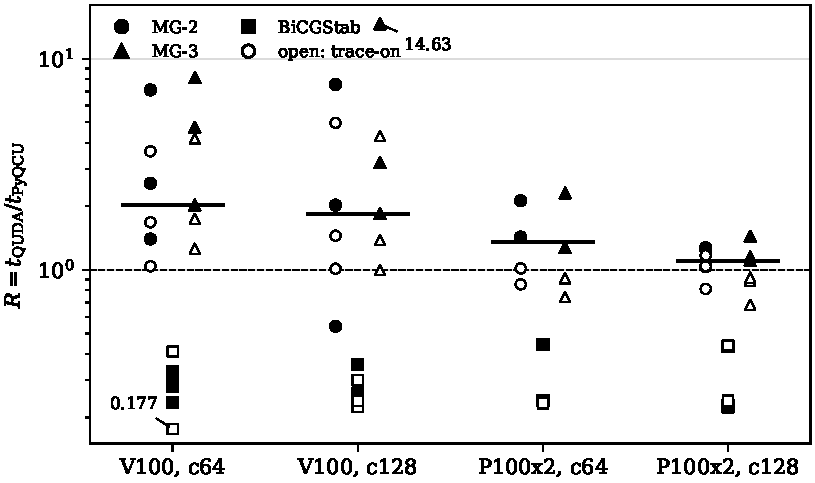
\includegraphics[width=0.96\linewidth]{High-Performance_Implementation_MG_assets/paper_assets/fig_ratio_distribution.pdf}
\caption{66 个精确单元的逐点时间比。实心符号为 trace-off，空心为
trace-on；水平短线为对应设备-精度组的 trace-off 中位数。极值是单点，
不表示置信区间。}
\label{fig:ratio-distribution}
\end{figure}

\subsection{设备与精度分组}

\begin{table}[htbp]
\centering
\caption{trace-off 分组中位时间比 \(R\)}
\label{tab:group-ratio}
\small
\begin{tabular}{@{}lrrrr@{}}
\toprule
设备/精度 & MG-2 & MG-3 & BiCGStab & 备注 \\
\midrule
V100 / c64 & 2.5717 & 4.7366 & 0.2818 & \(n=3\) \\
V100 / c128 & 2.0269 & 3.2174 & 0.2580 & \(n=3\) \\
P100\(\times2\) / c64 & 1.7773 & 1.7944 & 0.3416 & \(n=2\) \\
P100\(\times2\) / c128 & 1.2502 & 1.1517 & 0.2284 & \(n=3\) \\
\bottomrule
\end{tabular}
\end{table}

\begin{figure}[htbp]
\centering
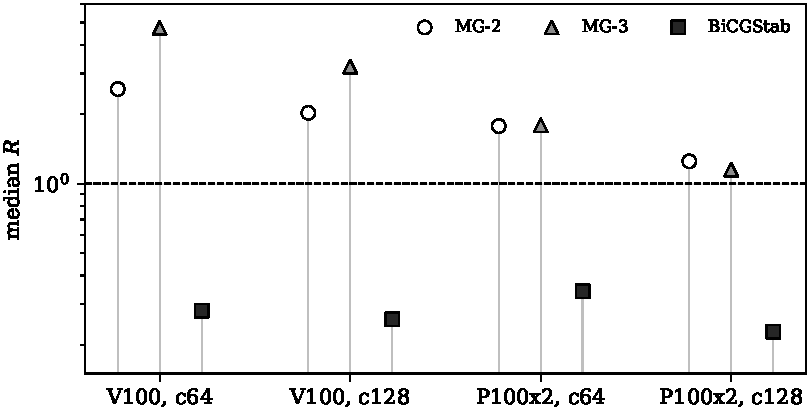
\includegraphics[width=0.92\linewidth]{High-Performance_Implementation_MG_assets/paper_assets/fig_group_medians.pdf}
\caption{trace-off 条件下各设备、精度和求解器的中位时间比。}
\label{fig:group-medians}
\end{figure}

V100 上的 MG 优势最明显，V100 c64 MG-3 与 c128 MG-3 的分组中位
时间比分别为 4.74 和 3.22。双 P100 的 MG-2/3 中位数均大于 1，
但幅度较小。分组极值表明结果对格点体积和残差轨迹敏感：
V100 c128 MG-3 的最大单点为 14.63，而 V100 c128 MG-2 中存在
0.54 的慢点。因此不能以单一最大值代表设备性能。

\subsection{阶段归因与容量边界}

\begin{table}[htbp]
\centering
\caption{trace-on MG 阶段耗时份额中位数}
\label{tab:stage-share}
\small
\begin{tabular}{@{}lrrrrrr@{}}
\toprule
实现 & pre & post & restrict & prolong & coarse & other \\
\midrule
PyQCU & 2.1\% & 2.0\% & 0.5\% & 0.5\% & 43.9\% & 50.9\% \\
QUDA & 10.5\% & 17.3\% & 1.0\% & 0.7\% & 69.3\% & 0.1\% \\
\bottomrule
\end{tabular}
\end{table}

\begin{figure}[htbp]
\centering
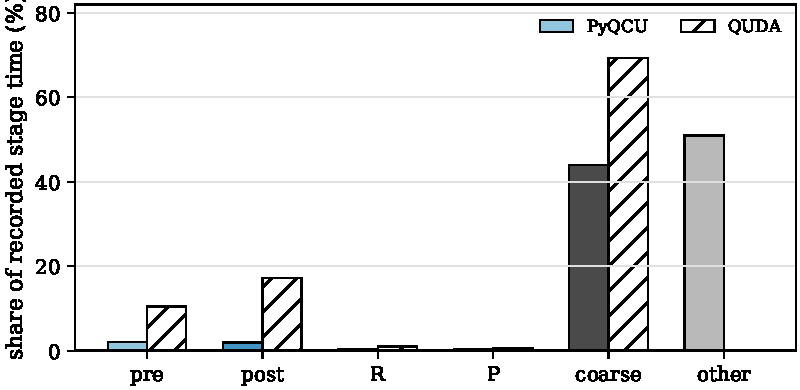
\includegraphics[width=0.88\linewidth]{High-Performance_Implementation_MG_assets/paper_assets/fig_stage_shares.pdf}
\caption{recorded stage time 的中位数份额。两侧层级映射不同，
只能比较各自的总时间结构，不能把同名阶段跨实现直接相加。}
\label{fig:stage-share}
\end{figure}

PyQCU 的 trace 记录中，coarse solve 与 \code{other} 合计约占 95\%；
QUDA 的主要成本集中在具名 coarse 阶段。由于两侧层级映射不同，
\code{other} 与同名列不能直接跨库比较。该结果说明后续优化应首先
聚焦粗层求解、同步、残差检查和通信，而不是继续优化细层算术。

双 P100 的 \code{c64}
\(16\times32\times32\times48\) 请求项未进入精确矩阵。三次尝试为：
默认 overlap 路径峰值约 15.9 GB，占设备容量 93.1\%；
\code{PYQCU_MPI_OVERLAP=0} 为 14.8 GB，占 86.2\%；
extended CPU-staging 降至 12.4 GB，占 72.4\%，但 MG-2 setup
仍超过 570 s。对应 6 个 combined 项被显式替代为 \(16^4\)，
并单独记录，未伪装成原格点性能。

\subsection{残差与显存}

\begin{table}[htbp]
\centering
\caption{精确矩阵的最大 full true residual 与 device-wide 峰值显存}
\label{tab:resource}
\small
\begin{tabular}{@{}lrrr@{}}
\toprule
实现 & 样本 & 最大真残差 & 最大观测显存 \\
\midrule
PyQCU & 66 & \(7.40\times10^{-7}\) & 11907.3 MiB \\
QUDA & 66 & \(7.97\times10^{-7}\) & 23063.3 MiB \\
\bottomrule
\end{tabular}
\end{table}

\begin{figure}[htbp]
\centering
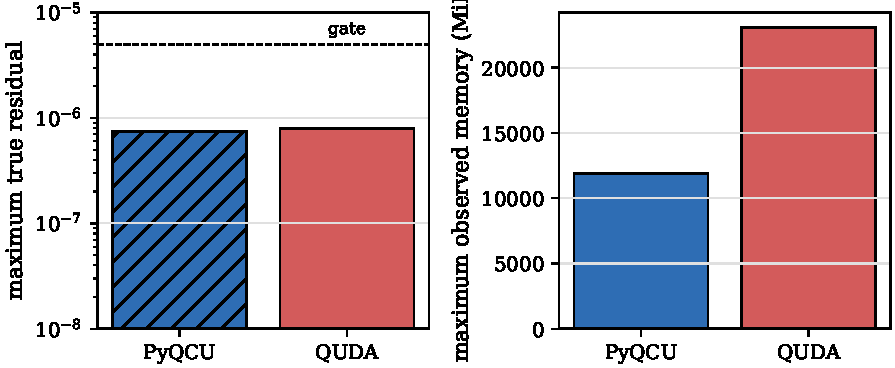
\includegraphics[width=0.92\linewidth]{High-Performance_Implementation_MG_assets/paper_assets/fig_residual_memory.pdf}
\caption{最大真残差与 device-wide 最大观测显存。显存 sampler 可能包含
同设备上的其他进程，因此用于容量门限检查，不声明为进程独占峰值。}
\label{fig:resource}
\end{figure}

两种实现的最大真残差均远低于 \(5\times10^{-6}\) 门限。保留样本的
最大 device-wide 显存均低于 85\% 门限，其中 PyQCU 的最大观测值约为
QUDA 的一半。该比较必须结合设备和格点分组理解，不能单独推断
所有配置下的内存效率。

\section{讨论}

\subsection{优势}

\begin{enumerate}
  \item \textbf{MG 专项性能明确。} 在 66 个精确单元中，MG-2/3
        为 35/44 有利；trace-off MG 为 21/22 有利。
  \item \textbf{V100 场景优势显著。} V100 c64/c128 MG-3
        trace-off 分组中位比分别为 4.74 和 3.22。
  \item \textbf{结构扁平、自主可控。} 求解器、Cython 桥、C++ ABI、
        CUDA 内核和测试矩阵位于同一仓库，便于针对 Clover--Wilson
        迭代和增加新功能。
  \item \textbf{资源与正确性证据完整。} 配置哈希、输入 bundle、
        1/2/5 phase、阶段时间、真残差、显存和容量替代均保留原始记录。
\end{enumerate}

\subsection{局限}

\begin{enumerate}
  \item 66 个精确单元的总中位仅为 1.025，整体优势较弱。
  \item BiCGStab reference 为 0/22 有利，说明优势来自 MG，而不是
        所有线性求解器。
  \item trace-on 引入明显同步开销，部分双 P100 分组退到 1 以下。
  \item 双 P100 c64 大格触发显存或 570 s setup 限制，必须使用
        显式容量替代。
  \item complex128 distributed overlap 改变浮点累加顺序，默认关闭；
        link halo 仍使用阻塞通信。
  \item 当前证据主要覆盖 V100 单卡和双 P100，不能外推到任意拓扑或
        千卡级 MPI。
\end{enumerate}

\subsection{后续工作}

后续工作按优先级分为四类：
\begin{enumerate}
  \item 将 coarse solve、残差检查和全局归约的同步进一步合并；
  \item 扩展 device-aware MPI、持久 request 和可选 NVSHMEM 通信；
  \item 降低 setup 峰值显存，使大格 c64/c128 可进入正式矩阵；
  \item 将稳定的 Python/ABI 回归扩展到更多作用量、混合精度和国产
        加速器后端。
\end{enumerate}

\section{结论}

本文给出了 PyQCU 中面向 Wilson--Clover 费米子的高性能 MultiGrid
实现，并从算子定义、低模粗空间、Galerkin 投影、CUDA--C++ 优化和
性能对照五个层面进行了分析。Strict 路径使用
\(D=X+H\)、\(\widehat D=X^{-1}D\) 和
\(D_{l+1}=R\widehat DP\)，在保持完整 Clover 物理语义的同时，
将低模误差转移到粗层。CUDA--C++ 后端通过矩阵自由/打包资产、
设备端标量、流重叠、融合内核、图执行、显存预算、原子缓存和
非阻塞 halo 降低真实 wall time。

\code{test27} 的最终数据说明：
\begin{enumerate}
  \item 66 个精确单元全部通过 config、input 和真残差门；
  \item MG-2/3 在 35/44 个单元中优于 QUDA，trace-off MG 为
        21/22；
  \item V100 上的 MG 优势最明显，双 P100 在 trace-off 下总体有利；
  \item 未完成的 6 个双 P100 c64 大格请求项被明确替代，没有混入
        公平加速比；
  \item PyQCU 的最大真残差和最大观测显存均满足预设门限。
\end{enumerate}
因此，当前实现可作为一个结构扁平、自主可控并且在典型 MG 场景
接近国际先进实现的求解器原型。下一阶段的决定性问题是粗层同步、
通信重叠、setup 显存和更大规模拓扑，而不是继续扩大小格或单点
加速比。

\appendix

\section{复现接口}

\begin{verbatim}
source ./env.sh
bash ./build.sh
bash ./install.sh

python -B pyqcu/testing/qcu/strict/quda_comparison/run_strict_fast.py \
  --fail-fast --json strict-fast.json

mpirun -np 2 python -B \
  pyqcu/testing/qcu/strict/quda_comparison/strict_mpi_solve_probe.py \
  --shape 8 8 8 16 --grid 2 1 1 1 --dtype c64 \
  --galerkin-mode colored

python -B pyqcu/testing/qcu/strict/quda_comparison/bench_mg_matrix_full.py \
  --list
\end{verbatim}

正式矩阵、侧记录、聚合和报告生成入口分别为
\pathref{bench_mg_matrix_full.py}、
\pathref{bench_strict_vs_quda.py}、
\pathref{assemble_final_matrix.py} 和
\pathref{build_mg_report.py}。

\section{原始证据索引}

\begin{longtable}{@{}L{0.34\textwidth}L{0.58\textwidth}@{}}
\caption{最终性能证据文件}\\
\toprule
文件 & 内容 \\
\midrule
\endfirsthead
\toprule
文件 & 内容 \\
\midrule
\endhead
\pathref{units.csv} & 66 个精确单元的总时间、迭代数、真残差和显存 \\
\pathref{stages.csv} & 逐层 pre/post/R/P/coarse/other 阶段记录 \\
\pathref{references.csv} & BiCGStab cold/warmup/steady 原始样本 \\
\pathref{requested_matrix_status.csv} & 72 个请求单元的精确或替代状态 \\
\pathref{capacity_substitutions.csv} & 6 个双 P100 c64 大格替代记录 \\
\pathref{summary_analysis.json} & 覆盖、分组和残差汇总 \\
\pathref{mg_memory.csv} & 逐 side 显存原始记录 \\
\pathref{mg_residual_curves.pdf} & trace-on 收敛曲线 \\
\pathref{mg_stage_breakdown.pdf} & 逐层阶段堆叠图 \\
\bottomrule
\end{longtable}

\begin{thebibliography}{9}

\bibitem{wilson}
K. G. Wilson,
\newblock Confinement of quarks,
\newblock \emph{Physical Review D} \textbf{10}, 2445 (1974).
\newblock \url{https://doi.org/10.1103/PhysRevD.10.2445}

\bibitem{clover}
B. Sheikholeslami and R. Wohlert,
\newblock Improved continuum limit lattice action for QCD with Wilson fermions,
\newblock \emph{Nuclear Physics B} \textbf{259}, 572 (1985).
\newblock \url{https://doi.org/10.1016/0550-3213(85)90002-1}

\bibitem{adaptive-mg}
R. Babich, J. Brannick, R. C. Brower, M. A. Clark,
T. A. Manteuffel, S. F. McCormick, J. C. Osborn, and C. Rebbi,
\newblock Adaptive multigrid algorithm for the lattice Wilson--Dirac operator,
\newblock \emph{Physical Review Letters} \textbf{105}, 201602 (2010).
\newblock \url{https://doi.org/10.1103/PhysRevLett.105.201602}

\bibitem{quda-paper}
M. A. Clark, R. Babich, K. Barros, R. C. Brower, and C. Rebbi,
\newblock Solving lattice QCD systems of equations using mixed precision
solvers on GPUs,
\newblock \emph{Computer Physics Communications} \textbf{181}, 1517 (2010).
\newblock \url{https://doi.org/10.1016/j.cpc.2010.05.002}

\bibitem{quda}
QUDA Collaboration,
\newblock QUDA: A library for lattice QCD computations on GPUs.
\newblock \url{https://github.com/lattice/quda}

\bibitem{ddalpha}
M. Rottmann et al.,
\newblock DD-$\alpha$AMG: Adaptive algebraic multigrid for lattice QCD.
\newblock \url{https://github.com/mrottmann/DDalphaAMG}

\bibitem{quantum-mg}
E. Weinberg,
\newblock quantum-mg: Multigrid solver package for lattice QCD.
\newblock \url{https://github.com/weinbe2/quantum-mg}

\bibitem{pyqcu}
张鑫,
\newblock PyQCU: Python/Cython and CUDA--C++ lattice QCD toolkit.
\newblock \url{https://github.com/zhangxin8069/PyQCU}

\end{thebibliography}

\end{document}
